

% Gradient Info
  
\tikzset {_9ett5n0d2/.code = {\pgfsetadditionalshadetransform{ \pgftransformshift{\pgfpoint{0 bp } { 0 bp }  }  \pgftransformrotate{-90 }  \pgftransformscale{2 }  }}}
\pgfdeclarehorizontalshading{_kkttfrljg}{150bp}{rgb(0bp)=(0.96,0.96,0.96);
rgb(37.5bp)=(0.96,0.96,0.96);
rgb(51.875bp)=(0.87,0.87,0.89);
rgb(100bp)=(0.87,0.87,0.89)}
\tikzset{every picture/.style={line width=0.75pt}} %set default line width to 0.75pt        

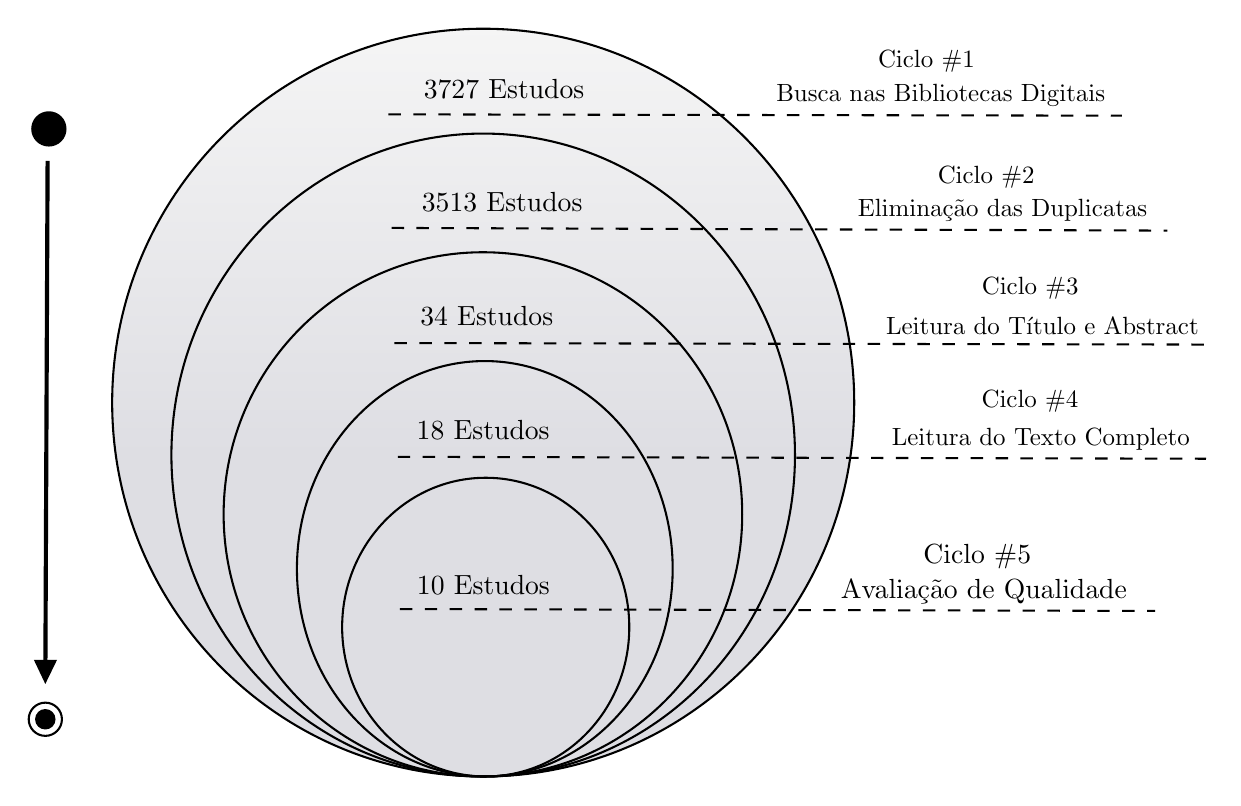
\begin{tikzpicture}[x=0.75pt,y=0.75pt,yscale=-1,xscale=1]
%uncomment if require: \path (0,423); %set diagram left start at 0, and has height of 423

%Flowchart: Connector [id:dp2928546604203144] 
\path  [shading=_kkttfrljg,_9ett5n0d2] (53.5,191.87) .. controls (53.5,92.38) and (133.53,11.73) .. (232.26,11.73) .. controls (330.98,11.73) and (411.02,92.38) .. (411.02,191.87) .. controls (411.02,291.35) and (330.98,372) .. (232.26,372) .. controls (133.53,372) and (53.5,291.35) .. (53.5,191.87) -- cycle ; % for fading 
 \draw   (53.5,191.87) .. controls (53.5,92.38) and (133.53,11.73) .. (232.26,11.73) .. controls (330.98,11.73) and (411.02,92.38) .. (411.02,191.87) .. controls (411.02,291.35) and (330.98,372) .. (232.26,372) .. controls (133.53,372) and (53.5,291.35) .. (53.5,191.87) -- cycle ; % for border 

%Flowchart: Connector [id:dp4856968141430813] 
\draw   (82.04,217.12) .. controls (82.04,131.59) and (149.3,62.25) .. (232.26,62.25) .. controls (315.22,62.25) and (382.47,131.59) .. (382.47,217.12) .. controls (382.47,302.66) and (315.22,372) .. (232.26,372) .. controls (149.3,372) and (82.04,302.66) .. (82.04,217.12) -- cycle ;
%Flowchart: Connector [id:dp8496211285519002] 
\draw   (107.2,245.72) .. controls (107.2,175.97) and (163.13,119.43) .. (232.13,119.43) .. controls (301.12,119.43) and (357.05,175.97) .. (357.05,245.72) .. controls (357.05,315.46) and (301.12,372) .. (232.13,372) .. controls (163.13,372) and (107.2,315.46) .. (107.2,245.72) -- cycle ;
%Flowchart: Connector [id:dp6739952869493944] 
\draw   (142.51,271.93) .. controls (142.51,216.66) and (183.04,171.85) .. (233.03,171.85) .. controls (283.02,171.85) and (323.55,216.66) .. (323.55,271.93) .. controls (323.55,327.2) and (283.02,372) .. (233.03,372) .. controls (183.04,372) and (142.51,327.2) .. (142.51,271.93) -- cycle ;
%Flowchart: Connector [id:dp626524831544014] 
\draw   (164.3,300.04) .. controls (164.3,260.3) and (195.27,228.08) .. (233.47,228.08) .. controls (271.67,228.08) and (302.64,260.3) .. (302.64,300.04) .. controls (302.64,339.78) and (271.67,372) .. (233.47,372) .. controls (195.27,372) and (164.3,339.78) .. (164.3,300.04) -- cycle ;
%Straight Lines [id:da31235038530795767] 
\draw  [dash pattern={on 4.5pt off 4.5pt}]  (186.61,52.99) -- (539.94,53.63) ;


%Straight Lines [id:da5536929778572981] 
\draw  [dash pattern={on 4.5pt off 4.5pt}]  (188.12,107.71) -- (561.94,109) ;


%Straight Lines [id:da6737369833612874] 
\draw  [dash pattern={on 4.5pt off 4.5pt}]  (189.5,163.17) -- (583.25,163.91) ;


%Straight Lines [id:da5470247173512306] 
\draw  [dash pattern={on 4.5pt off 4.5pt}]  (191.11,217.99) -- (580.5,218.91) ;


%Straight Lines [id:da665185906632269] 
\draw  [dash pattern={on 4.5pt off 4.5pt}]  (192.11,291.33) -- (555.98,292.25) ;


%Straight Lines [id:da29299456740910346] 
\draw [line width=1.5]    (22.39,75.43) -- (21.3,324.43) ;
\draw [shift={(21.29,327.43)}, rotate = 270.25] [fill={rgb, 255:red, 0; green, 0; blue, 0 }  ][line width=1.5]  [draw opacity=0] (11.61,-5.58) -- (0,0) -- (11.61,5.58) -- cycle    ;

%Flowchart: Connector [id:dp48946546663936763] 
\draw  [fill={rgb, 255:red, 0; green, 0; blue, 0 }  ,fill opacity=1 ] (15,60) .. controls (15,55.58) and (18.58,52) .. (23,52) .. controls (27.42,52) and (31,55.58) .. (31,60) .. controls (31,64.42) and (27.42,68) .. (23,68) .. controls (18.58,68) and (15,64.42) .. (15,60) -- cycle ;
%Flowchart: Connector [id:dp24133340263386382] 
\draw   (13.29,344.43) .. controls (13.29,340.01) and (16.87,336.43) .. (21.29,336.43) .. controls (25.7,336.43) and (29.29,340.01) .. (29.29,344.43) .. controls (29.29,348.85) and (25.7,352.43) .. (21.29,352.43) .. controls (16.87,352.43) and (13.29,348.85) .. (13.29,344.43) -- cycle ;
%Flowchart: Connector [id:dp2687972500754565] 
\draw  [fill={rgb, 255:red, 0; green, 0; blue, 0 }  ,fill opacity=1 ] (16.87,344.43) .. controls (16.87,341.99) and (18.85,340.01) .. (21.29,340.01) .. controls (23.72,340.01) and (25.7,341.99) .. (25.7,344.43) .. controls (25.7,346.87) and (23.72,348.85) .. (21.29,348.85) .. controls (18.85,348.85) and (16.87,346.87) .. (16.87,344.43) -- cycle ;

% Text Node
\draw (445.81,27.26) node [scale=0.9] [align=left] {Ciclo \#1};
% Text Node
\draw (452.7,43.84) node [scale=0.9] [align=left] {Busca nas Bibliotecas Digitais};
% Text Node
\draw (474.6,83.22) node [scale=0.9] [align=left] {Ciclo \#2};
% Text Node
\draw (495.84,136.68) node [scale=0.9] [align=left] {Ciclo \#3};
% Text Node
\draw (495.72,191.35) node [scale=0.9] [align=left] {Ciclo \#4};
% Text Node
\draw (470.32,265.86) node [scale=1] [align=left] {Ciclo \#5};
% Text Node
\draw (242.31,40.79) node [scale=1] [align=left] {3727 Estudos};
% Text Node
\draw (482.49,99.04) node [scale=0.9] [align=left] {Eliminação das Duplicatas};
% Text Node
\draw (241.4,94.97) node [scale=1] [align=left] {3513 Estudos};
% Text Node
\draw (501.67,155.11) node [scale=0.9] [align=left] {Leitura do Título e Abstract};
% Text Node
\draw (233.99,150.1) node [scale=1] [align=left] {34 Estudos};
% Text Node
\draw (500.9,209.51) node [scale=0.9] [align=left] {Leitura do Texto Completo};
% Text Node
\draw (232.26,205.21) node [scale=1] [align=left] {18 Estudos};
% Text Node
\draw (473.47,282.92) node [scale=1] [align=left] {Avaliação de Qualidade};
% Text Node
\draw (232.38,279.6) node [scale=1] [align=left] {10 Estudos};


\end{tikzpicture}
